% !TEX root = 1_memoire.tex
\section*{Introduction}
La transcription automatique de la musique (AMT) est un défi ancien
\cite{first_one} et difficile qui n’est toujours pas résolu. Il a engendré une
pluie de sous-tâches qui ont donné naissance au domaine de la recherche
d’information musicale (MIR). Actuellement, de nombreux travaux de MIR font
appel au traitement automatique des langues (TAL) \footnote{NLP4MuSA, the 2nd
Workshop on Natural Language Processing for Music and Spoken Audio, co-located
with ISMIR 2021.}.\\
Dans ce chapitre, nous parlerons de l’informatique musicale, nous tenterons
d’établir les liens existants entre le MIR et le TAL ainsi qu’entre les notions
de langage musical et langue naturelle. Nous traiterons également de l’utilité
et du problème de l’AMT et de la transcription automatique de la batterie
(ADT).\\
Enfin, nous décrirons les représentations de la musique qui sont nécessaires à
la compréhension du présent travail.
\section{TAL et MIR}
L'informatique musicale \cite{mus_inf} est une étude du traitement de la
musique \cite{book_muller}, en particulier des représentations musicales, de la
transformée de Fourier pour la musique \cite{fourier}, de l'analyse de la
structure de la musique et de la reconnaissance des accords\footnote{En
musique, un accord est un ensemble de notes considéré comme formant un tout du
point de vue de l'harmonie. Le plus souvent, ces notes sont jouées
simultanément ; mais les accords peuvent aussi s'exprimer par des notes
successives}. D'autres sujets de recherche en informatique musicale comprennent
la modélisation informatique de la musique, l'analyse informatique de la
musique, la reconnaissance optique de la musique, les éditeurs audio
numériques, les moteurs de recherche de musique en ligne, la recherche
d'informations musicales et les questions cognitives dans la musique.\\
Le MIR\footnote{https://ismir.net/} apparaît vers le début des années 2000
\cite{MIR_1}. C’est une science interdisciplinaire qui fait appel à de nombreux
domaines comme la musicologie, l’analyse musicale, la psychologie, les sciences
de l’information, le traitement du signal et les méthodes d’apprentissage
automatisé en informatique. Cette discipline récente a notamment été soutenue
par de grandes compagnies du web\footnote{\url{https://research.deezer.com/}}
\footnote{\url{https://magenta.tensorflow.org/}}
\footnote{\url{https://research.atspotify.com/}} qui veulent développer des
systèmes de recommandation de musique ou des moteurs de recherche dédiés au son
et à la musique.\\\\
\begin{figure}[!h]
	\centering
	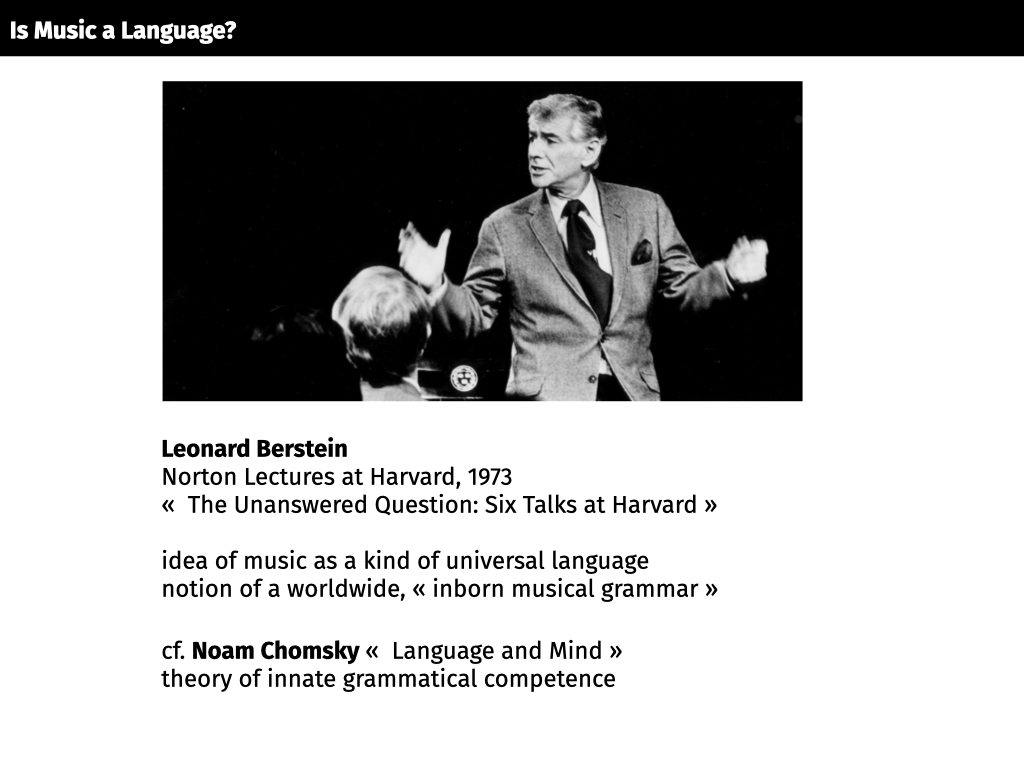
\includegraphics[height=85mm, width=120mm]{z_images/1_contexte/0_Bernstein.png}
\end{figure}\\
Aborder la musique à travers le TAL nécessite une réflexion autour de la
musique en tant que langage ainsi que la possibilité de comparer ce même
langage avec les langues naturelles. Quelques travaux en neurosciences ont
abordé la question, notamment par observation des processus cognitifs et
neuronaux que les systèmes de traitement de ces deux langages avaient en
commun. Dans le travail de Poulin-Charronnat \textit{et al.}
\cite{poulincharronnat:hal-01985213}, la musique est reconnue comme étant un
système complexe spécifique à l’être humain dont une des similitudes avec les
langues naturelles est l’émergence de régularités reconnues implicitement par
le système cognitif. La question de la pertinence de l’analogie entre langues
naturelles et langage musical a également été soulevée à l’occasion de projets
de recherche en TAL. Keller \textit{et al.} \cite{keller:hal-03279850} ont
exploré le potentiel de ces techniques à travers les plongements de mots et le
mécanisme d’attention pour la modélisation de données musicales. La question du
sens d’une phrase musicale apparaît, selon eux, à la fois comme une limite et
un défi majeur pour l’étude de cette analogie.\\\\
% \textit{Ici, Digression sur la musicologie calculatoire vs linguistique computationnelle ?}\\\\
D’autres travaux très récents, ont aussi été révélés lors de la
\textit{première conférence sur le NLP pour la musique et l'audio
(NLP4MusA 2020)}. Lors de cette conférence, Jiang \textit{et al.}
\cite{Jiang2020DiscoveringMR} ont présenté leur implémentation d’un modèle de
langage musical auto-attentif visant à améliorer le mécanisme d'attention par
élément, déjà très largement utilisé dans les modèles de séquence modernes pour
le texte et la musique.\\
Le domaine du TAL qui se rapproche le plus du MIR est la reconnaissance de la
parole (Speech to text). En effet, la séparation des sources ont des approches similaires dans
les deux domaines. De plus, il existe un lien entre partition musicale comme
manière d’écrire la musique et texte comme manière d’écrire la parole.\\\\
\begin{table}[h]
	\centering
	\begin{tabular}{|c|c|c|} \hline
		Domaines & Similitudes & Différences \\ \hline
		Speech to text & signal $\Rightarrow$ phonèmes $\Rightarrow$ texte & données linéaires\\
		AMT & signal $\Rightarrow$ MIDI $\Rightarrow$ partition & données structurées\\ \hline
	\end{tabular}
	\caption{speechToText vs AMT}
	\label{spToTxt_vs_AMT}
\end{table}
\section{La transcription automatique de la musique}
En musique, la transcription\footnote{\url{
https://en.wikipedia.org/wiki/Transcription_(music)}} est la pratique
consistant à noter un morceau ou un son qui n'était auparavant pas noté et/ou pas populaire en tant que musique écrite, par exemple, une improvisation de jazz ou une bande sonore de jeu vidéo. Lorsqu'un musicien est chargé de créer une partition à partir d'un enregistrement et qu'il écrit les notes qui composent le morceau en notation musicale, on dit qu'il a créé une transcription musicale de cet enregistrement.\\
L'objectif de la transcription automatique de la musique (AMT) \cite{future_directions} est de convertir la performance d'un musicien en notation musicale - un peu comme la conversion de la parole en texte dans le traitement du langage naturel. L’AMT a des intérêt multiples, notamment pour la transcription de solos ou encore pour la constitution de corpus musicologiques, ou encore pour l'interprétation de la musique et l'analyse du contenu musical \cite{SHIBATA2021262}. Par exemple, un grand nombre de fichiers audio et vidéo musicaux sont disponibles sur le Web, et pour la plupart d'entre eux, il est difficile de trouver les partitions musicales correspondantes, qui sont nécessaires pour pratiquer la musique, faire des reprises et effectuer une analyse musicale détaillée. Les partitions de musique classique sont facilement accessibles et il y a peu de demandes de nouvelles transcriptions. D'un point de vue pratique, des demandes beaucoup plus commerciales et académiques sont attendues dans le domaine de la musique populaire \cite{SHIBATA2021262}. Les modèles grammaticaux qui représentent la structure hiérarchique des séquences d'accords se sont avérés très utiles dans les analyses récentes de l'harmonie du jazz \cite{harasimjazz}.
Comme déjà évoqué précédemment, il s’agit d’un problème ancien et difficile. C’est un « graal » de l’informatique musicale. En 1976, H. C. Longuet-Higgins \cite{first_one} évoquait déjà la représentation musicale en arbre syntaxique dans le but d’écrire automatiquement des partitions à partir de données audio en se basant sur un mimétisme psychologique de l’approche humaine. De même pour les chercheurs en audio James A. Moorer, Martin Piszczalski et Bernard Galler qui, en 1977\footnote{\url{https://en.wikipedia.org/wiki/Transcription_(music)}}, ont utilisé leurs connaissances en ingénierie de l’audio et du numérique pour programmer un ordinateur afin de lui faire analyser un enregistrement musical numérique de manière à détecter les lignes mélodiques, les accords et les accents rythmiques des instruments à percussion.\\
La tâche de transcription automatique de la musique comprend deux activités distinctes : l'analyse d'un morceau de musique et l'impression d'une partition à partir de cette analyse.\\\\
La figure \ref{AMT_presentation} est une proposition de Benetos \textit{et al.} \cite{future_directions} qui représente l'architecture générale d'un système de transcription musicale. On y observe plusieurs sous-tâches de l’AMT :
\begin{itemize}
	\item La séparation des sources à partir de l’audio.
	\item Le système de transcription :
	\begin{itemize}
		\item Cœur du système :\\
		$\Rightarrow$ Algorithmes de détection des multi-pitchs et de suivi des \tab notes.\\
		Quatres sous-tâches optionnelles accompagnent ces algorithmes :
		\begin{itemize}
			\item identification de l'instrument ;
			\item estimation de la tonalité et de l'accord ;
			\item détection de l'apparition et du décalage ;
			\item estimation du tempo et du rythme.
		\end{itemize}
	\end{itemize}
	\item Apprentissage sur des modèles accoustiques et musicologiques.
	\item \textit{Optionnel :} Informations fournies de manière externe, soit fournie en amont (genre, instruments,…), soit par interaction avec un utilisateur (infos sur une partition incomplète).
\end{itemize}
\begin{figure}[!h]
	\centering
	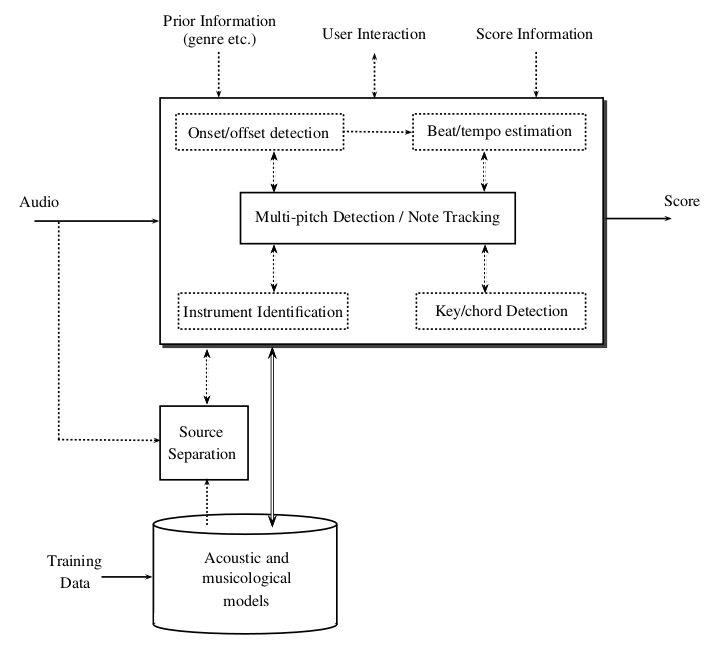
\includegraphics[height=95mm, width=130mm]{z_images/1_contexte/1_general_process.png}
	\caption{Transcription automatique}
	\label{AMT_presentation}
	\textit{Les sous-systèmes et algorithmes optionnels sont présentés à l'aide de lignes pointillées. Les doubles flèches mettent en évidence les connexions entre les systèmes qui incluent la fusion d'informations et une communication plus interactive entre les systèmes.}
\end{figure} %\newpage
\florent{éviter newpage}

\section{La transcription automatique de la batterie}
\florent{tres bonne section}
La batterie est un instrument récent qui s’est longtemps passé de partition. En effet pour un batteur, la qualité de lecteur lorsqu’elle était nécessaire, résidait essentiellement dans sa capacité à lire les partitions des autres instrumentistes (par exemple, les grilles d’accords et la mélodie du thème en jazz) afin d’improviser un accompagnement approprié que personne ne pouvait écrire pour lui à sa place.

Les partitions de batterie sont arrivées par nécessité avec la pédagogie et l’émergence d’écoles de batterie partout dans le monde. 
\florent{cite méthode et école Agostini ?}
Un autre facteur qui a contribué à l’expansion des partitions de batterie est l’émergence de la musique assistée par ordinateur (MAO). En effet, l’usage de boîtes à rythmes ou de séquenceurs permettant d’expérimenter soi-même l’écriture de rythmes en les écoutant mixés avec d’autres instruments sur des machines a permis  aux compositeurs de s’émanciper de la création d’un batteur en lui fournissant une partition contenant les parties exactes qu’ils voulaient entendre sur leur musique.\\
La batterie a un statut à part dans l’univers de l’AMT puisqu'il s'agit d'instruments sans hauteur (du point de vue harmonique), d'événements sonores auxquels une durée est rarement attribuée et de notations spécifiques (symboles des têtes de notes).
\florent{citer \cite{Review_ADT} ici}

Les applications de l’ADT seraient utiles dans tous les domaines musicaux 
\florent{ADT pas défini}
contenant de la batterie dont certains manque de partitions, 
\florent{"contenant" -> concernés par}
notamment les musiques d’improvisation (jazz, pop) \cite{future_directions}.
%
Mais aussi de manière plus générale dans le domaine du MIR. 
\florent{manque verbe}
Si les ordinateurs étaient capables d'analyser la partie de la batterie dans la musique enregistrée, 
cela permettrait 
\florent{permettrait de faciliter}
une variété de tâches de traitement de la musique liées au rythme. En particulier, la détection et la classification des événements sonores de la batterie par des méthodes informatiques est considérée comme un problème de recherche important et stimulant dans le domaine plus large de la recherche d'informations musicales \cite{Review_ADT}.

L'ADT est un sujet de recherche crucial pour la compréhension des aspects rythmiques de la musique, et a un impact potentiel sur des domaines plus larges tels que l'éducation musicale et la production musicale.

\section{Les représentations de la musique}
\florent{citer M. Müller FMP pour cette section?}

\subsection*{Les données audio}
\florent{trop technique. ne pas recopier wikipédia}
Le fichier WAV\footnote{https://en.wikipedia.org/wiki/WAV} est une instance du Resource Interchange File Format (RIFF) défini par IBM et Microsoft. 
Le format RIFF agit comme une "enveloppe" pour divers formats de codage audio.
Bien qu'un fichier WAV puisse contenir de l'audio compressé, 
le format audio WAV le plus courant est l'audio non compressé au format LPCM (linear pulse-code modulation). 
\florent{LPCM pas utile ici. parle juste échantillons et compression.}
Le LPCM est également le format de codage audio standard des CD audio, qui stockent des données audio LPCM à deux canaux échantillonnées à 44 100 Hz avec 16 bits par échantillon. Comme le LPCM n'est pas compressé et conserve tous les échantillons d'une piste audio, les utilisateurs professionnels ou les experts en audio peuvent utiliser le format WAV avec l'audio LPCM pour obtenir une qualité audio maximale.
\florent{tu peux mentionner le format spectral (analyse harmonique) crucial en MIR audio.}

\subsection*{Les données MIDI}
Le MIDI\footnote{\url{https://en.wikipedia.org/wiki/MIDI}} (Musical Instrument Digital Interface) 
\florent{ne pas copier wikipédia verbatim. source: midi.org
         MIDI est un protocole temps réel pour échanger des messages (événement) et un format de fichier.}
est une norme technique qui décrit un protocole de communication, une interface numérique et des connecteurs électriques permettant de connecter une grande variété d'instruments de musique électroniques, d'ordinateurs et d'appareils audio connexes pour jouer, éditer et enregistrer de la musique.

\florent{fichier MIDI = séquence événements MIDI + dates (timestamp) ~ performance musicale symbolique}
\florent{donner ici les données des événements et expliquer ON/OFF (clavier)}
Les données midi sont représentées sous forme de piano-roll. 
%
Chaque point sur la figure \ref{piano_roll} est appelé « évènement MIDI » :
\begin{figure}[!h]
	\centering
	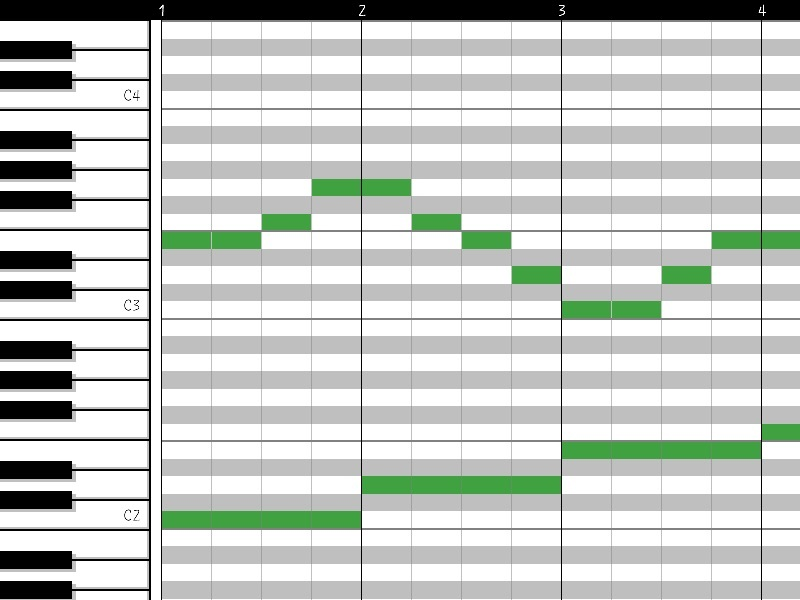
\includegraphics[height=40mm, width=50mm]{z_images/1_contexte/2_midi_piano.jpg}
	\caption{Exemple évènements avec durée}
	\label{piano_roll}
\end{figure}

Chaque évènement MIDI rassemble un ensemble d’informations sur la hauteur, la durée, le volume, etc… :
\begin{figure}[h!]
	\centering
	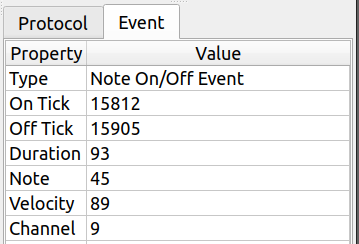
\includegraphics[height=40mm, width=50mm]{z_images/1_contexte/3_evenements_midi.png}
	\caption{Critère pour un évènement}
\end{figure} %\newpage
\florent{il n'y a pas de duration d'événement dans un MIDI file. 
         la "durée" est une distance entre 2 événemtns ON et OFF (c'est important dans ton travail).
         le screenshot n'est pas utile, écrit plutôt une liste itemize}

Pour la batterie, les évènements sont considérés sans durée, nous ignorerons donc les offsets (« Off Event »), les « Off Tick » et les « Duration ». Le \textit{channel} ne nous sera pas utile non plus.\\
\textit{Ici, définir Tick et channel.}

Voici un exemple de piano-roll midi pour la batterie :
\begin{figure}[h!]
	\centering
	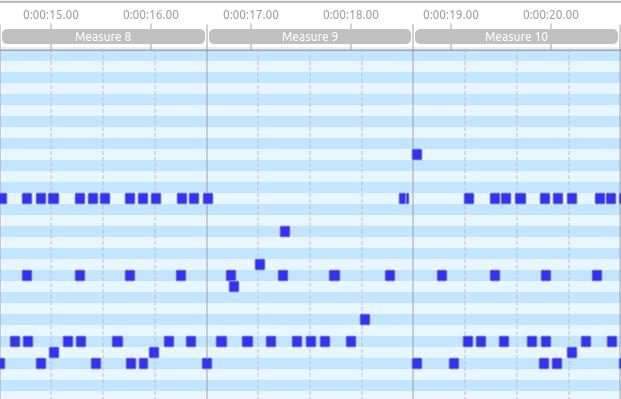
\includegraphics[height=40mm, width=50mm]{z_images/1_contexte/4_midi_batterie.png}
	\caption{Exemple évènements sans durée}
\end{figure}

On observe que toutes les durées sont identiques.
\subsection*{Les partitions}
\begin{figure}[h!]
	\centering
	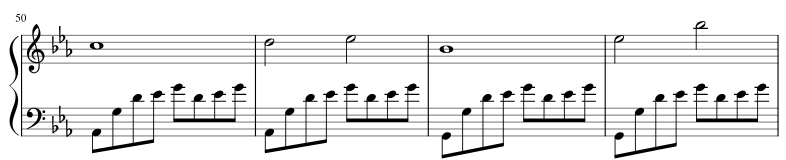
\includegraphics[height=30mm, width=120mm]{z_images/1_contexte/5_partition_piano.png}
	\caption{Exemple de partition de piano}
\end{figure}

Une partition de musique\footnote{\url{https://fr.wikipedia.org/wiki/Partition\_(musique)}} est un document qui porte la représentation systématique du langage musical sous forme écrite. Cette représentation est appelée transcription et elle sert à traduire les quatre caractéristiques du son musical :
\begin{itemize}
	\item la hauteur ;
	\item la durée ;
	\item l'intensité ;
	\item le timbre.
\end{itemize}
\florent{expliquer un peu plus avec exemple. 
ce serait mieux d'avoir un ex. avec des nuances, accents, appogiatures...}

Ainsi que de leurs combinaisons appelées à former l'ossature de l'œuvre musicale dans son déroulement temporel, à la fois :
\begin{itemize}
	\item diachronique (succession des instants, ce qui constitue en musique la mélodie) ;
	\item et synchronique (simultanéité des sons, c'est-à-dire l'harmonie).
\end{itemize}
\florent{explications sur l'aspect structuré (hiérarchie) : les mesures, les groupes ryhtmiques...
         c'est important ici}

\subsection*{Le format MusicXML}
\florent{existe plusieurs formats XML: MusicXML, MEI, MNX, qui sont autant de schemas XML}
MusicXML est un format de fichier basé sur XML pour représenter la notation musicale occidentale. Ce format est ouvert, entièrement documenté et peut être utilisé librement dans le cadre de l'accord de spécification finale de la communauté du W3C.
\florent{standard W3C = MNX (en cours)}

Un des avantages de ce format est qu’il peut être converti aussi bien en données MIDI qu’en partition musicale, ce qui en fait une interface homme/machine.

\begin{figure}[h]
	\centering
	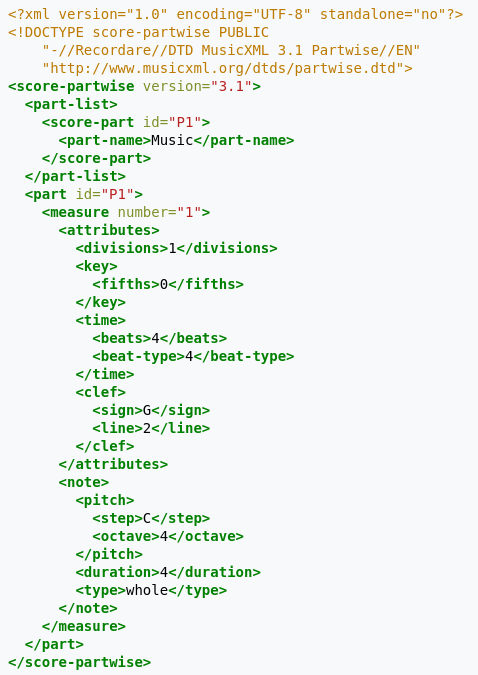
\includegraphics[height=80mm, width=70mm]{z_images/1_contexte/6_musicxml.png}
	\caption{MusicXML}
	\label{MusicXML}
\end{figure}

Le figure \ref{MusicXML} représente un do en clef de sol de la durée d’une ronde sur une mesure en 4/4.
\florent{inconvénient: format.s verbeux et ambigus. 
         -> on utilise pour la transcription une représentation intermédiaire abstraite décrite plus loin.}


\section*{Conclusion}
Dans ce chapitre, nous avons établi que le MIR s’intéresse de plus en plus au TAL, et que, par ce biais, il y a des liens possibles entre le langage musical et les langues naturelles, le plus proche étant probablement le phénomène d’écriture des sons de l’un comme de l’autre.\\
Nous avons également établi que le MIR est né de l’AMT qui est un problème ancien et très difficile et qu’il serait toujours très utile de le résoudre (autant pour l’AMT que pour l’ADT).\\
Et enfin, nous avons décrit les représentations de la musique nécessaires à la compréhension du présent mémoire, allant du son jusqu’à l’écriture.

